\documentclass{article}
\usepackage{tikz}
\usepackage{lscape}
\usepackage{makecell}
\usetikzlibrary{automata,positioning}
\usepackage{amsmath,amsfonts,amssymb}

\begin{document}

\section*{Advanced operations management - Simulation study}

\section{System of choice}
Approximation of the pump manufacturing process at GRUNDFOS.

\section{Reference model}
The following reference model is used as an approximation of the pump manufacturing process.
\begin{itemize}
    \item Entity: Raw components (metal sheets)
    \item Resource machines: Cutting, Ring assembly, Pipe assembly, Cleaning, Pump assembly
    \item Activity: Produce pumps from raw components
    \item Events: Entity arrival (external), resource jobs finish (internal)
    \item States:\\
        $Q_1$: queue at cutting machine \\
        $B_1$: number of busy cutting machines \\
        $Q_2$: queue at ring assembly \\
        $B_2$: number of busy ring assembly \\
        $Q_3$: queue at pipe assembly \\
        $B_3$: number of busy pipe assembly \\
        $Q_4$: queue at cleaning machine \\
        $B_4$: number of busy cleaning machines \\
        $Q_5$: queue at assembly line \\
        $B_5$: number of busy pump assembly\\
        $B_i$Max: Maximum number of servers at machine $i$, for $i=1,...,5$
    \item State transition: We transition to a new state whenever an event happens.
\end{itemize}

\newpage
\begin{landscape}
~
\vfill
\begin{figure}[h]
    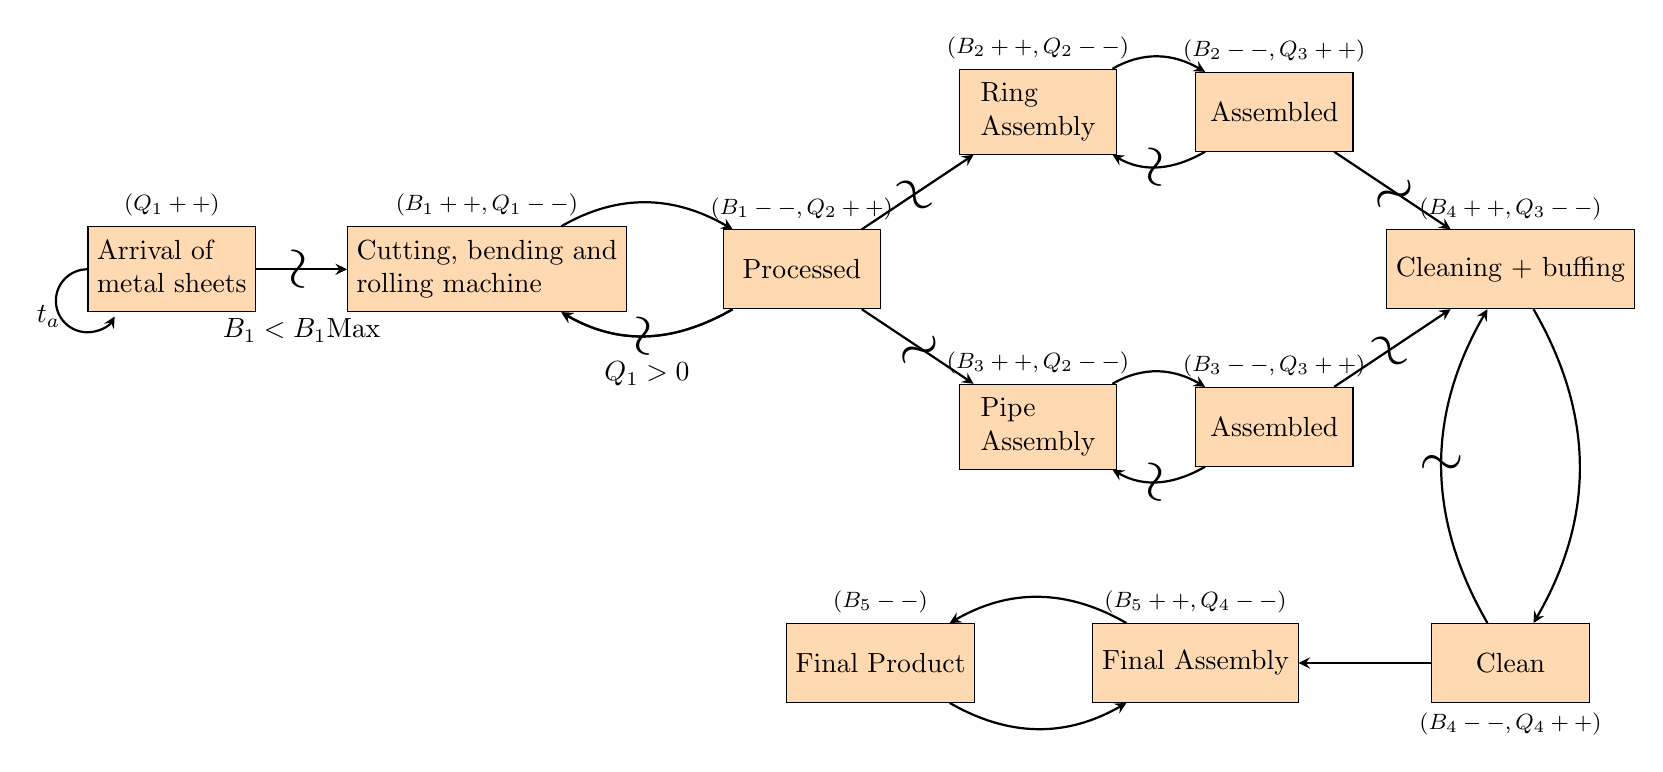
\begin{tikzpicture}[node distance = 3cm]
        \tikzstyle{process} = [rectangle, minimum width=2cm, minimum height=1cm, text centered, draw=black, fill=orange!30]
        \tikzstyle{arrow} = [thick,->,>=stealth]
        \tikzstyle{arrow_invisible} = [thick,->,>=stealth,line width=0pt]
        
        % nodes
        \node (arrival) [process, label=above:{\footnotesize($Q_1++$)}] {\makecell[l]{Arrival of\\metal sheets}};
        \node (preprocess) [process, right of=arrival, xshift=1cm, label=above:{\footnotesize($B_1++,Q_1--$)}] {\makecell[l]{Cutting, bending and\\rolling machine}};
        \node (processed) [process, right of=preprocess, xshift=1cm, label=above:{\footnotesize($B_1--,Q_2++$)}] {Processed};
        \node (ring) [process, right of=processed, yshift=2cm, label=above:{\footnotesize($B_2++,Q_2--$)}] {\makecell[l]{Ring\\Assembly}};
        \node (pipe) [process, right of=processed, yshift=-2cm, label=above:{\footnotesize($B_3++,Q_2--$)}] {\makecell[l]{Pipe\\Assembly}};
        \node (ring_asmbl) [process, right of=ring, label=above:{\footnotesize($B_2--,Q_3++$)}] {Assembled};
        \node (pipe_asmbl) [process, right of=pipe, label=above:{\footnotesize($B_3--,Q_3++$)}] {Assembled};
        \node (cleaning) [process, right of=ring_asmbl,yshift=-2cm, label=above:{\footnotesize($B_4++,Q_3--$)}] {Cleaning + buffing};
        \node (clean) [process, below of=cleaning, yshift=-2cm, label=below:{\footnotesize($B_4--, Q_4++$)}] {Clean};
        \node (final_assembly) [process, left of=clean, xshift=-1cm, label=above:{\footnotesize($B_5++, Q_4--$)}] {Final Assembly};
        \node (final_prod) [process, left of=final_assembly,xshift=-1cm, label=above:{\footnotesize($B_5--$)}] {Final Product};
        
        % arrows
        \draw [arrow] (arrival.180) arc (90:330:4mm) node[midway]{$t_a\;\;
        \;$};
        \draw[arrow_invisible] (arrival) -- node[midway, rotate=90] {\huge$\sim$} (preprocess);
        \draw[arrow] (arrival) -- node[below,yshift=-.5cm] {$B_1< B_1$Max}(preprocess);
        \draw [arrow] (preprocess) to [out=30,in=150] (processed);
        \draw [arrow] (processed) to [out=-150,in=-30] node[midway, rotate=90] {\huge$\sim$} (preprocess);
        \draw [arrow] (processed) to [out=-150,in=-30] node[below, yshift=-.2cm] {$Q_1>0$} (preprocess);
        \draw [arrow] (processed) -- node[midway, rotate=135] {\huge$\sim$}(ring);
        \draw [arrow] (processed) -- node[midway, rotate=205] {\huge$\sim$}(pipe);
        \draw [arrow] (ring) to [out=30,in=150] (ring_asmbl);
        \draw [arrow] (ring_asmbl) to [out=-150,in=-30]  node[midway, rotate=90] {\huge$\sim$} (ring);
        \draw [arrow] (pipe) to [out=30,in=150] (pipe_asmbl);
        \draw [arrow] (pipe_asmbl) to [out=-150,in=-30]  node[midway, rotate=90] {\huge$\sim$} (pipe);
        \draw [arrow] (ring_asmbl) -- node[midway, rotate=205] {\huge$\sim$} (cleaning);
        \draw [arrow] (pipe_asmbl) -- node[midway, rotate=135] {\huge$\sim$} (cleaning);
        \draw [arrow] (cleaning) to [out=-60,in=60] (clean);
        \draw [arrow] (clean) to [out=-240,in=-120] node[midway] {\huge$\sim$} (cleaning);
        \draw [arrow] (clean) -- (final_assembly);
        \draw [arrow] (final_assembly) to [out=150,in=30] (final_prod);
        \draw [arrow] (final_prod) to [out=-30,in=-150] (final_assembly);
        
    \end{tikzpicture}
    \caption{Petrinet}
\end{figure}
\end{landscape}

\vfill

\end{document}
